\begin{figure}[H]
    \begin{center}
      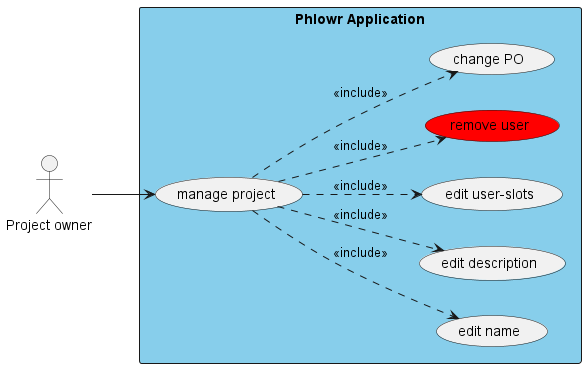
\includegraphics[width=0.3\linewidth]{../content/diagrams/usecase/manageProject/manageProjectUseCaseRemoveUserSelected.png}
      \caption{Use Case Diagaramm <remove user> }
    \end{center}
  \end{figure}

  \begin{table}[H]
    \centering
    \settowidth\tymin{executeIncomingCommand()}
    \setlength\extrarowheight{2pt}
    \begin{tabulary}{1.0\textwidth}{|m{4cm}|m{9cm}|}
      \hline
      \textbf{Use Case} &
      \textbf{REMOVE USER}\\
      \hline
      \textbf{Beschreibung} &
      Ein User wird aus einem Projekt entfernt\\ 
      \hline
      \textbf{Includes} &
      \begin{itemize}
       \item keine
        \end{itemize}\\
        \hline  
      \textbf{Akteure} &
      Projekt-Owner\\ 
      \hline
      \textbf{Auslöser} &
      \begin{itemize}
        \item ein Entwickler arbeitet nicht mehr am Projekt
        \item ein Entwickler hat fälschlicherweise beim Projekt registriert
         \end{itemize}\\  
      \hline
      \textbf{Vorbedingungen} &
      \begin{itemize}
        \item Vorbedingungen vom <manage project>-Use-Case
        \item Der zu entfernende User hat sich als Entwickler beim Projekt registriert
        \item Die vorhandenen Tasks des Users wurden vorgängig bereinigt
      \end{itemize}\\  
      \hline
      \textbf{Abschlussbedingunen} &
      Der User ist nicht mehr im Projekt registriert\\ 
      \hline
      \textbf{Ablauf} &
      \begin{enumerate}
        \item Applikation öffnen
        \item <Projekt Editieren> wählen
        \item unter dem Abschnitt <Entwickler> wird der entsprechende User geöffnet
        \item <Entwickler entfernen> wird gewählt
        \item Speichern
        \end{enumerate}\\ 
      \hline
      \textbf{Zu Beachten / Notizen} &
      \begin{itemize}
        \item wird ein User entfernt, so müssen allfällige Kommentare des Users in den Tasks usw. entsprechend berücksichtigt werden
        \end{itemize}\\ 
      \hline
    \end{tabulary}
    \caption{Use Case: manage project -> remove user}
  \end{table}
